% ==========================================================================
% Defensa TFM - data.lung  ·  10 slides · ~10 min
% Estructura: motivación + método + resultados + DEMO app + conclusiones
% ==========================================================================
\documentclass[aspectratio=169, 11pt]{beamer}

\usepackage[utf8]{inputenc}
\usepackage[T1]{fontenc}
\usepackage[spanish]{babel}
\shorthandoff{".<>}
\usepackage{lmodern}
\usepackage{amssymb}
\usepackage{booktabs}
\usepackage{tikz}
\usepackage{graphicx}
\usepackage{xcolor}
\usetikzlibrary{arrows.meta, positioning, calc, shapes.geometric}

% -------- Tema minimal editorial --------
\usetheme{default}
\useinnertheme{default}
\useoutertheme{default}
\setbeamertemplate{navigation symbols}{}
\setbeamertemplate{itemize items}{\color{verdeTerm}$\blacktriangleright$}
\setbeamertemplate{itemize subitem}{\color{verdeTerm}\textbullet}

\definecolor{verdeTerm}{HTML}{1C8A3F}
\definecolor{verdeOsc}{HTML}{146A2F}
\definecolor{ambar}{HTML}{C78A1E}
\definecolor{tinta}{HTML}{0B0B0B}
\definecolor{tinta2}{HTML}{4A4948}
\definecolor{mute}{HTML}{8F8D87}
\definecolor{plano}{HTML}{F7F4EB}
\definecolor{linea}{HTML}{DAD6C8}

% Colores de marca de las tecnologías (para las badges)
\definecolor{pythonAzul}{HTML}{306998}
\definecolor{pythonAmarillo}{HTML}{FFD43B}
\definecolor{githubGris}{HTML}{24292F}
\definecolor{streamlitRojo}{HTML}{FF4B4B}
\definecolor{ncbiAzul}{HTML}{205493}
\definecolor{latexVerde}{HTML}{008080}
\definecolor{groqNaranja}{HTML}{F55036}
\definecolor{llamaVioleta}{HTML}{6B4EFF}
\definecolor{sklearnAzul}{HTML}{F7931E}
\definecolor{tcgaAzul}{HTML}{1F4E79}

\setbeamercolor{normal text}{fg=tinta}
\setbeamercolor{frametitle}{fg=tinta}
\setbeamercolor{title}{fg=tinta}
\setbeamercolor{structure}{fg=verdeTerm}
\setbeamerfont{frametitle}{series=\bfseries, size=\large}
\setbeamerfont{title}{series=\bfseries, size=\LARGE}

% Barra inferior (una sola linea, texto corto, sin desbordes)
\setbeamertemplate{footline}{%
  \hbox to \paperwidth{%
    \hspace*{1em}%
    {\ttfamily\scriptsize\color{verdeTerm}\textbf{>}\;\color{tinta2}data\textcolor{verdeTerm}{.}lung}%
    \hspace{0.8em}{\color{mute}\scriptsize\textbullet}\hspace{0.8em}%
    {\scriptsize\color{tinta2}Daniel Tapia D\'iez \textperiodcentered\ TFM UAX}%
    \hfill%
    {\scriptsize\color{mute}\insertframenumber\,/\,\inserttotalframenumber}%
    \hspace*{1em}%
  }%
  \vspace{4pt}%
}

% Reservar espacio para el footer al calcular el area de contenido
\setbeamersize{text margin left=1em, text margin right=1em}

% T\'itulo de cada slide con filete verde (compacto)
\setbeamertemplate{frametitle}{%
  \vspace{0.7em}%
  \hspace{0.5em}\insertframetitle\\[-4pt]%
  \hspace{0.5em}\textcolor{verdeTerm}{\rule{1.2cm}{2pt}}%
  \vspace{-0.8em}%
}

% ------------- Badges de tecnologías -------------
\graphicspath{{./}{logos/}}

% Logo real desde PNG, altura consistente
\newcommand{\logoImg}[2][0.8cm]{%
  \raisebox{-0.15\height}{\includegraphics[height=#1]{#2}}%
}

% Badge de texto (fallback cuando no hay logo oficial)
\newcommand{\techbadge}[2]{%
  \tikz[baseline=(N.base)]{
    \node[fill=#1, text=white, rounded corners=3pt,
          inner xsep=6pt, inner ysep=3pt,
          font=\ttfamily\bfseries\footnotesize] (N) {#2};
  }%
}

\newcommand{\gene}[1]{\textit{#1}}
\newcommand{\kicker}[1]{{\ttfamily\small\color{verdeTerm}\textbf{>} #1}}
\newcommand{\bignum}[1]{{\fontsize{40pt}{40pt}\selectfont\color{verdeTerm}\textbf{#1}}}
\newcommand{\mednum}[1]{{\fontsize{28pt}{28pt}\selectfont\color{verdeTerm}\textbf{#1}}}
\newcommand{\lbl}[1]{{\ttfamily\scriptsize\color{mute}\MakeUppercase{#1}}}

\title{Framework transcriptómico para biomarcadores en cáncer de pulmón}
\author{Daniel Tapia Díez}
\date{14 de agosto de 2026}

% ==========================================================================
\begin{document}

% =============== SLIDE 1: PORTADA CON STACK TECNOLÓGICO ===================
{\setbeamertemplate{footline}{}
\begin{frame}[plain]
  \vspace{-0.1cm}
  \begin{center}
    
\includegraphics[width=2.4cm]{logouax1.png}\\[0.25cm]

    {\ttfamily\fontsize{44pt}{44pt}\selectfont\bfseries
     data\textcolor{verdeTerm}{.}lung}\\[0.05cm]
    {\itshape\small\color{tinta2}Del dataset a una firma génica replicable}\\[0.25cm]

    \textcolor{verdeTerm}{\rule{2cm}{1.5pt}}\\[0.2cm]
    {\bfseries\small\color{tinta}
      Framework transcriptómico basado en la integración de
      modelos de lenguaje y aprendizaje automático\\
      para la identificación de biomarcadores en cáncer de pulmón}\\[0.4cm]

    {\small\color{tinta}\textbf{Daniel Tapia Díez}}\;\;
    {\scriptsize\color{mute}$\cdot$}\;\;
    {\scriptsize\color{tinta2}Tutor: Leonardo Dulcetti}\;\;
    {\scriptsize\color{mute}$\cdot$}\;\;
    {\scriptsize\color{tinta2}14 ago 2026}\\[0.3cm]

    % Stack tecnológico (logos oficiales)
    {\ttfamily\scriptsize\color{mute}CONSTRUIDO CON}\\[0.2cm]
    \logoImg[0.7cm]{python.png}\hspace{0.6cm}%
    \logoImg[0.55cm]{sklearn.png}\hspace{0.6cm}%
    \logoImg[0.6cm]{streamlit.png}\hspace{0.6cm}%
    \logoImg[0.55cm]{meta.png}\hspace{0.6cm}%
    \techbadge{groqNaranja}{Groq}\hspace{0.6cm}%
    \logoImg[0.7cm]{github.png}\\[0.3cm]
    {\ttfamily\scriptsize\color{mute}DATOS DE}\\[0.2cm]
    \logoImg[0.7cm]{ncbi.png}\hspace{0.9cm}%
    \logoImg[0.55cm]{cbioportal.png}
  \end{center}
\end{frame}
}

% =============== SLIDE 2: PROBLEMA + OBJETIVO =============================
\begin{frame}{El problema · el objetivo}
  \vspace{0.05cm}
  \begin{columns}[T]
    \column{0.5\textwidth}
    \kicker{Cáncer de pulmón}\\[0.15cm]
    {\fontsize{38pt}{38pt}\selectfont\color{verdeTerm}\textbf{2{,}48\,M}}\;{\footnotesize casos/año}\\[0.15cm]
    {\fontsize{30pt}{30pt}\selectfont\color{verdeTerm}\textbf{$<$20\,\%}}\;{\footnotesize superv. 5 años}\\[0.25cm]

    {\small Distinguir \textbf{adenocarcinoma} (ADC) de
    \textbf{carcinoma escamoso} (SQC) es crítico:
    pemetrexed y bevacizumab \textbf{contraindicados}
    en escamoso.}

    \column{0.5\textwidth}
    \kicker{El reto}\\[0.15cm]
    {\small Cientos de estudios GEO públicos, pero:
    \begin{itemize}\setlength\itemsep{1pt}
      \item Plataformas heterogéneas
      \item Metadatos en \textbf{texto libre}
      \item Firmas publicadas que \textbf{no replican}
    \end{itemize}}

    \vspace{0.25cm}
    \kicker{Objetivo}\\[0.1cm]
    {\itshape\small\color{verdeOsc}Framework reproducible que integra
    cohortes GEO con \textbf{curación LLM}, \textbf{validación LODO}
    y \textbf{firma consenso interpretable}.}
  \end{columns}
\end{frame}

% =============== SLIDE 3: PIPELINE ========================================
\begin{frame}{Método · pipeline de 9 pasos}
  \vspace{0.05cm}
  \begin{columns}[c]
    \column{0.55\textwidth}
    \begin{center}
      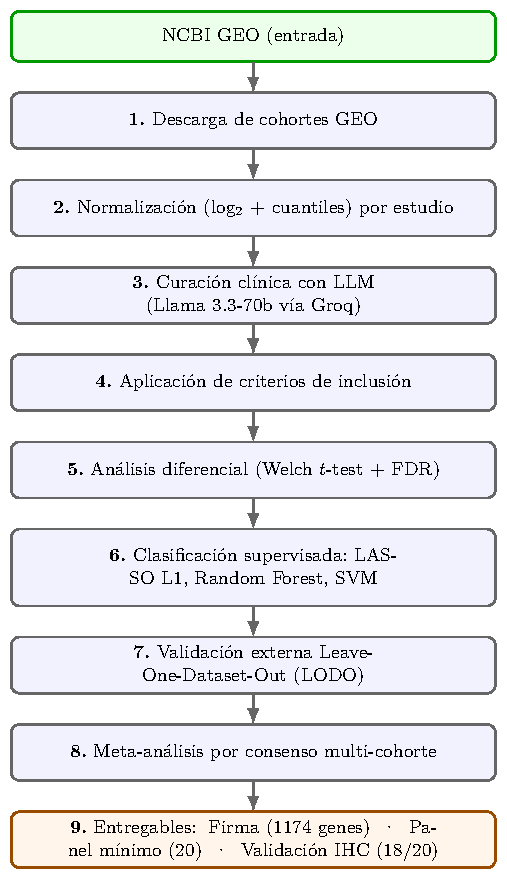
\includegraphics[height=0.68\textheight]{pipeline.pdf}
    \end{center}

    \column{0.45\textwidth}
    \kicker{Piezas clave}\\[0.15cm]
    {\small
    \begin{itemize}\setlength\itemsep{4pt}
      \item \textbf{Paso 3 · LLM}\\
      Llama 3.3-70b cura los metadatos clínicos de texto libre.
      Tasa de éxito \textbf{85,9\,\%}.

      \item \textbf{Paso 7 · LODO externa}\\
      Cada cohorte se retira una vez del entrenamiento
      y se usa como test independiente.

      \item \textbf{Paso 8 · Consenso multi-cohorte}\\
      Un gen entra en la firma sólo si mantiene signo y
      $|d| > 0{,}5$ en las 3 cohortes.
    \end{itemize}}

    \vspace{0.15cm}
    {\small\itshape\color{verdeOsc}Sin corrección de \emph{batch}:
    LODO no lo corrige, lo mide.}
  \end{columns}
\end{frame}

% =============== SLIDE 4: DATOS + FIRMA + PANEL ===========================
\begin{frame}{Resultados · firma génica y panel mínimo}
  \vspace{0.2cm}
  \begin{columns}[T]
    \column{0.32\textwidth}
    \bignum{11}\\\lbl{cohortes GEO}\\[0.4cm]
    \bignum{8/11}\\\lbl{cumplen criterios}\\[0.4cm]
    \bignum{1157}\\\lbl{muestras curadas LLM}

    \column{0.34\textwidth}
    \bignum{1174}\\\lbl{genes validados}\\
    \lbl{en 3 cohortes indep.}\\[0.4cm]
    \bignum{20}\\\lbl{genes panel mínimo}\\[0.4cm]
    \mednum{0{,}966}\;{\small vs 0,970}\\
    \lbl{auc panel · auc firma completa}

    \column{0.34\textwidth}
    \kicker{Top 5 firma}\\[0.15cm]
    {\small
    \begin{tabular}{@{}ll@{}}
      \gene{DSG3}   & desmosoma\\
      \gene{KRT5}   & queratina basal\\
      \gene{CALML3} & diferenciación\\
      \gene{KRT6B}  & queratina basal\\
      \gene{PKP1}   & desmosoma\\
    \end{tabular}}\\[0.4cm]

    {\small\itshape\color{verdeOsc}Los 20 del panel se pueden medir
    por PCR cuantitativa o \emph{NanoString}. Aplicable en clínica.}
  \end{columns}
\end{frame}

% =============== SLIDE 5: VALIDACION IHC + BIOLOGIA =======================
\begin{frame}{Resultados · validación externa contra IHC y biología}
  \vspace{0.2cm}
  \begin{columns}[T]
    \column{0.55\textwidth}
    \kicker{Panel diagnóstico OMS recuperado \textbf{sin declararlo}}\\[0.3cm]

    \begin{center}\small
      \begin{tabular}{@{}lc@{}}
        \toprule
        \textbf{Linaje} & \textbf{Recuperación} \\
        \midrule
        Escamoso        & \color{verdeTerm}\textbf{12 / 12} \\
        Adenocarcinoma  & \color{verdeTerm}\textbf{6 / 8} \\
        \midrule
        \textbf{Total}  & \color{verdeTerm}\textbf{18 / 20 · 90\,\%} \\
        \bottomrule
      \end{tabular}
    \end{center}

    \vspace{0.35cm}
    {\small\itshape\color{verdeOsc}Selección puramente estadística
    → coincide con el panel que ya usa la clínica.\\
    La firma no es sólo robusta: es \textbf{biológicamente correcta}.}

    \column{0.45\textwidth}
    \kicker{Interpretación · 2 ejes reales}\\[0.3cm]

    \textbf{Eje 1} · Pérdida alvéolo-capilar\\
    $\rho = -0{,}626$ media\\
    $\rho = -0{,}858$ en GSE31210 ($p=1{,}1\!\cdot\!10^{-66}$)\\[0.35cm]

    \textbf{Eje 2} · Actividad proliferativa\\
    {\small\gene{MKI67}, \gene{TOP2A}, \gene{CCNB1},
    \gene{BIRC5}, \gene{AURKA}}\\[0.4cm]

    \begin{center}\itshape\small\color{verdeOsc}
    La firma captura la transición\\
    del pulmón sano al tejido tumoral.
    \end{center}
  \end{columns}
\end{frame}

% =============== SLIDE 6: RENDIMIENTO + RECALIBRACION + TCGA ==============
\begin{frame}{Resultados · rendimiento, recalibración y RNA-Seq}
  \vspace{0.05cm}
  \begin{columns}[T]
    \column{0.5\textwidth}
    \kicker{LODO tumor vs sano · con recalibración}\\[0.15cm]

    \begin{center}\footnotesize
      \begin{tabular}{@{}lcc@{}}
        \toprule
        & \textbf{Sin recal.} & \textbf{Con isotónica} \\
        \midrule
        AUC          & 0,925 & 0,953 \\
        BalAcc       & 0,772 & \color{verdeTerm}\textbf{0,810} \\
        Sensibilidad & 0,983 & 0,988 \\
        Especificidad& 0,561 & \color{verdeTerm}\textbf{0,632} \\
        \bottomrule
      \end{tabular}
    \end{center}

    \vspace{0.15cm}
    \kicker{Comparativa LODO}\\[0.1cm]
    {\small LASSO 0,925 · RF 0,933 · SVM 0,957 (AUC)\\[0.05cm]
    LASSO elegido por interpretabilidad (coefs. por gen)}

    \column{0.5\textwidth}
    \kicker{Transferibilidad a RNA-Seq · TCGA}\\[0.15cm]

    {\small Panel entrenado en microarray → aplicado a\\
    \textbf{TCGA-LUAD} ($n=230$) + \textbf{TCGA-LUSC} ($n=178$)}

    \vspace{0.2cm}
    \bignum{0{,}857}\\\lbl{auc con score lasso transferido}\\[0.1cm]
    {\fontsize{22pt}{22pt}\selectfont\color{verdeTerm}\textbf{[0{,}812; 0{,}899]}}\\\lbl{ic 95\,\% bootstrap}\\[0.2cm]

    {\centering\itshape\footnotesize\color{verdeOsc}
      Ninguna muestra TCGA participó en la selección\\
      ni en la calibración. Plataforma cambiada,\\
      firma se transfiere.\par}
  \end{columns}
\end{frame}

% =============== SLIDE 7: DATA.LUNG (DEMO EN VIVO) ========================
\begin{frame}{data.lung · demo en vivo}
  \vspace{0.05cm}
  \begin{columns}[T]
    \column{0.5\textwidth}
    \kicker{Interfaz Streamlit multipágina}\\[0.1cm]
    {\footnotesize
    \begin{itemize}\setlength\itemsep{0pt}
      \item Portada + dashboard con 7 capítulos
      \item \textbf{Buscador de gen} sobre la firma
      \item Vista por cohorte (PCA, volcano, heatmap)
      \item Cifras leídas de los CSV — nada hardcoded
    \end{itemize}}

    \vspace{0.1cm}
    \kicker{Asistente Llama 3.3-70b acotado}\\[0.05cm]
    {\footnotesize
    \begin{itemize}\setlength\itemsep{0pt}
      \item Responde \emph{sólo} con los resultados del trabajo
      \item Reglas explícitas contra alucinación
      \item Distingue lo que está en la firma de lo que no
    \end{itemize}}

    \vspace{0.15cm}
    {\ttfamily\scriptsize\color{verdeTerm}\textbf{>}\;\color{tinta2}streamlit run paso12\_web\_chatbot.py}

    \column{0.5\textwidth}
    \vspace{-0.1cm}
    \begin{center}
      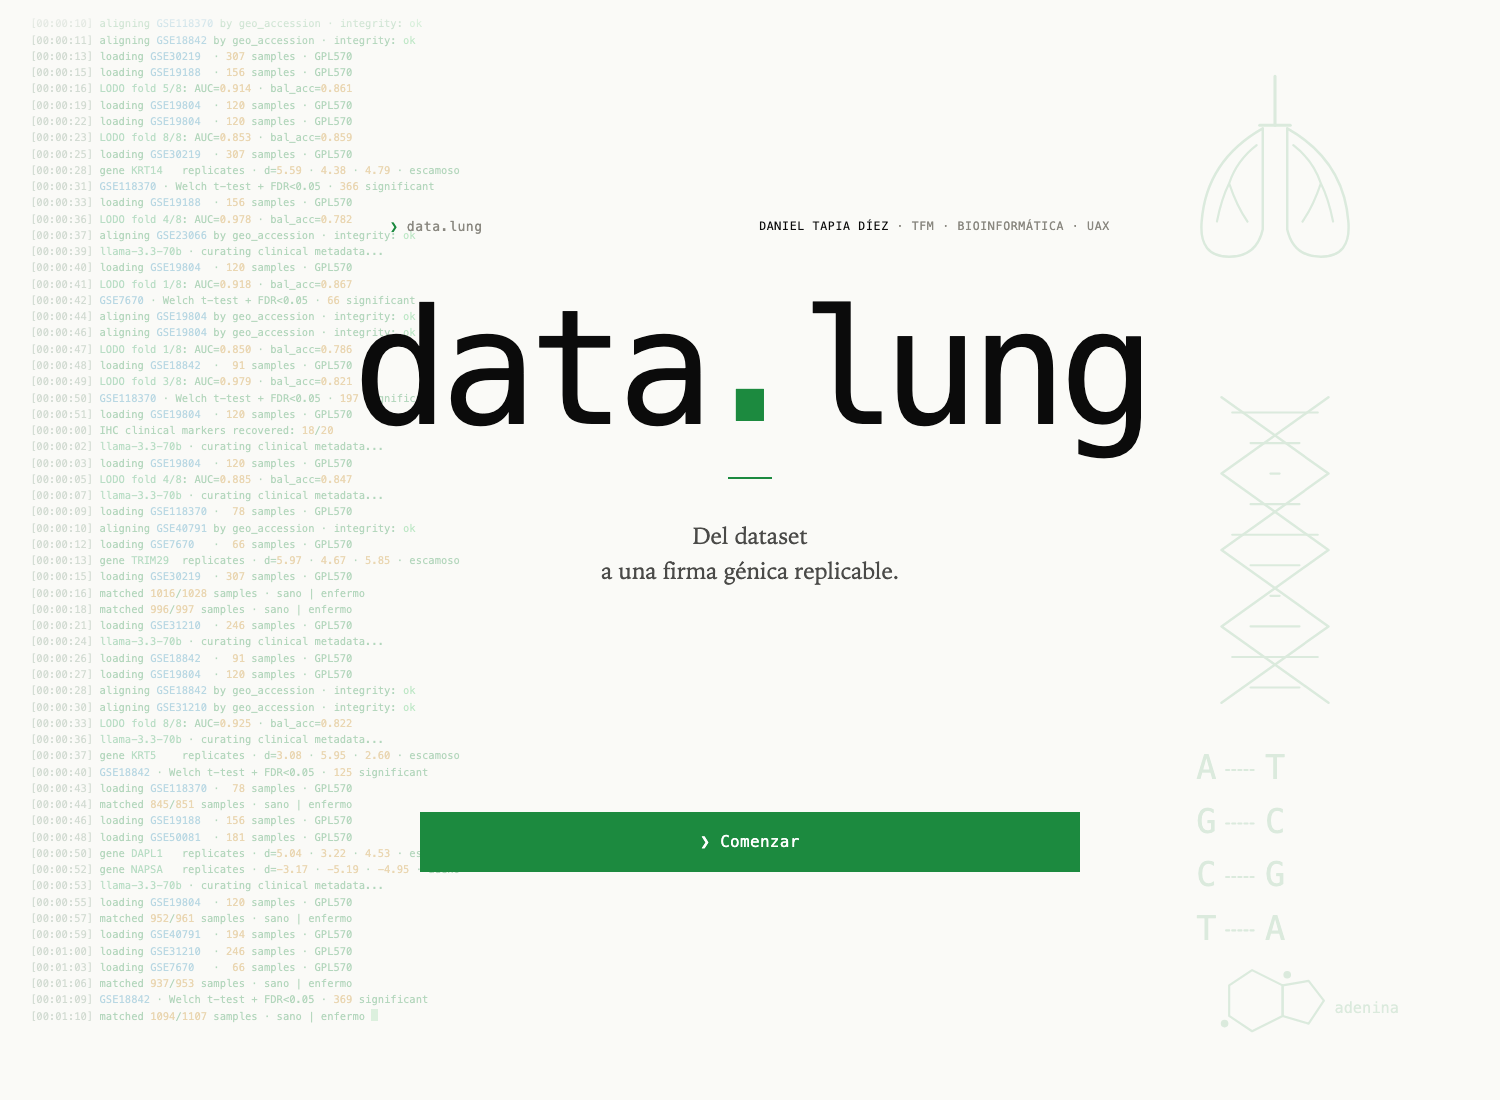
\includegraphics[width=\linewidth, height=0.75\textheight, keepaspectratio]{01_landing.png}\\[0.05cm]
      {\scriptsize\itshape\color{mute}(captura real $\cdot$ demo en vivo)}
    \end{center}
  \end{columns}
\end{frame}

% =============== SLIDE 8: CONCLUSIONES ====================================
\begin{frame}{Conclusiones}
  \vspace{0.05cm}
  {\small
  \begin{itemize}\setlength\itemsep{2pt}
    \item Un LLM cura los metadatos de GEO con \textbf{85,9\,\%} de éxito.

    \item Consenso multi-cohorte + LODO produce firma robusta:
    \textbf{1174 genes} con AUC \textbf{0,968} en subtipo.

    \item Panel mínimo de \textbf{20 genes} $\approx$ firma completa
    (0,966 vs 0,970), clínicamente manejable.

    \item La firma \textbf{recupera 18/20 marcadores IHC cl\'inicos} sin
    declararlos.

    \item Recalibración isotónica: \textbf{BalAcc 0,772 $\to$ 0,810}
    en tumor vs sano.

    \item El panel se transfiere a RNA-Seq: \textbf{AUC 0,857}
    en TCGA (408 muestras).

    \item Framework \textbf{reproducible} extremo a extremo con interfaz
    web y asistente acotado.
  \end{itemize}}
\end{frame}

% =============== SLIDE 9: TRABAJO FUTURO + STACK ==========================
\begin{frame}{Trabajo futuro · stack tecnológico}
  \vspace{0.05cm}
  \begin{columns}[T]
    \column{0.55\textwidth}
    \kicker{Líneas futuras}\\[0.15cm]
    {\small
    \begin{itemize}\setlength\itemsep{2pt}
      \item Validación clínica prospectiva sobre biopsias frescas
      (NanoString / RT-qPCR)
      \item Ampliación a subtipos neuroendocrinos
      \item Sustitución del LLM externo por modelo local
      \item Extensión metodológica a otros tumores
      (mama, colon, hepatocarcinoma)
      \item Firmas pronósticas (regresión de Cox sobre TCGA)
    \end{itemize}}

    \column{0.45\textwidth}
    \kicker{Reproducible sobre software libre}\\[0.2cm]
    \begin{center}
      \logoImg[0.65cm]{python.png}\hspace{0.5cm}\logoImg[0.55cm]{sklearn.png}\\[0.2cm]
      \logoImg[0.6cm]{streamlit.png}\hspace{0.5cm}\techbadge{groqNaranja}{Groq API}\\[0.2cm]
      \logoImg[0.55cm]{meta.png}\hspace{0.5cm}\logoImg[0.65cm]{ncbi.png}\\[0.2cm]
      \logoImg[0.55cm]{cbioportal.png}\hspace{0.5cm}\logoImg[0.55cm]{latex.png}\\[0.2cm]
      \logoImg[0.65cm]{github.png}
    \end{center}

    \vspace{0.1cm}
    \begin{center}{\ttfamily\tiny\color{mute}github.com/danitapiadiez-gif/TFM-Bioinformatica}\end{center}
  \end{columns}
\end{frame}

% =============== SLIDE 10: CIERRE =========================================
{\setbeamertemplate{footline}{}
\begin{frame}[plain]
  \vspace{1.2cm}
  \begin{center}
    {\ttfamily\fontsize{70pt}{70pt}\selectfont\bfseries
     data\textcolor{verdeTerm}{.}lung}\\[0.3cm]

    \textcolor{verdeTerm}{\rule{2cm}{2pt}}\\[0.4cm]

    {\Large\itshape\color{tinta2}Gracias por vuestra atención}\\[1cm]

    {\small\color{tinta2}Daniel Tapia Díez}\\[0.1cm]
    {\small\color{tinta2}Tutor: Leonardo Dulcetti · Universidad Alfonso X el Sabio}\\[0.4cm]
    {\ttfamily\small\color{mute}github.com/danitapiadiez-gif/TFM-Bioinformatica}
  \end{center}
\end{frame}
}

\end{document}
